\documentclass[12pt]{article}
\usepackage{pmmeta}
\pmcanonicalname{812TheClassicalProof}
\pmcreated{2013-11-06 2:20:56}
\pmmodified{2013-11-06 2:20:56}
\pmowner{PMBookProject}{1000683}
\pmmodifier{rspuzio}{6075}
\pmtitle{8.1.2 The classical proof}
\pmrecord{1}{}
\pmprivacy{1}
\pmauthor{PMBookProject}{6075}
\pmtype{Feature}
\pmclassification{msc}{03B15}

\endmetadata

\usepackage{xspace}
\usepackage{amssyb}
\usepackage{amsmath}
\usepackage{amsfonts}
\usepackage{amsthm}
\newcommand{\base}{\ensuremath{\mathsf{base}}\xspace}
\newcommand{\Sn}{\mathbb{S}}
\newcommand{\UU}{\ensuremath{\mathcal{U}}\xspace}
\newcommand{\Z}{\ensuremath{\mathbb{Z}}\xspace}
\let\autoref\cref
\let\type\UU
\begin{document}

\index{classical!homotopy theory|(}%
In classical homotopy theory, there is a standard proof of $\pi_1(\Sn^1)=\Z$ using universal covering spaces.
Our proof can be regarded as a type-theoretic version of this proof, with covering spaces appearing here as fibrations whose fibers are sets.
\index{fibration}%
\index{total!space}%
Recall that \emph{fibrations} over a space $B$ in homotopy theory correspond to type families $B\to\type$ in type theory.
\index{path!fibration}%
\index{fibration!of paths}%
In particular, for a point $x_0:B$, the type family $(x\mapsto (x_0=x))$ corresponds to the \emph{path fibration} $P_{x_0} B \to B$, in which the points of $P_{x_0} B$ are paths in $B$ starting at $x_0$, and the map to $B$ selects the other endpoint of such a path.
This total space $P_{x_0} B$ is contractible, since we can ``retract'' any path to its initial endpoint $x_0$ --- we have seen the type-theoretic version of this as \autoref{thm:contr-paths}.
Moreover, the fiber over $x_0$ is the loop space\index{loop space} $\Omega(B,x_0)$ --- in type theory this is obvious by definition of the loop space.

\begin{figure}\centering
  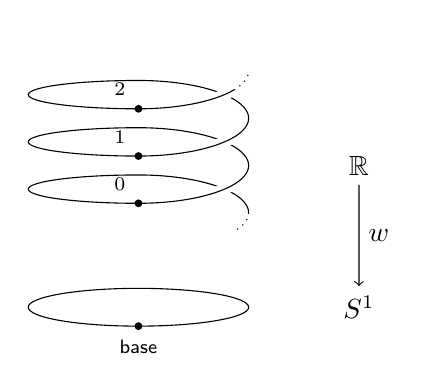
\begin{tikzpicture}[xscale=1.4,yscale=.6]
    \node (R) at (2,1) {$\mathbb{R}$};
    \node (S1) at (2,-2) {$S^1$};
    \draw[->] (R) -- node[auto] {$w$} (S1);
    \draw (0,-2) ellipse (1 and .4);
    \draw[dotted] (1,0) arc (0:-30:1 and .8);
    \draw (1,0) arc (0:90:1 and .8) arc (90:270:1 and .3) coordinate (t1);
    \draw[white,line width=4pt] (t1) arc (-90:90:1 and .8);
    \draw (t1) arc (-90:90:1 and .8) arc (90:270:1 and .3) coordinate (t2);
    \draw[white,line width=4pt] (t2) arc (-90:90:1 and .8);
    \draw (t2) arc (-90:90:1 and .8) arc (90:270:1 and .3) coordinate (t3);
    \draw[white,line width=4pt] (t3) arc (-90:90:1 and .8);
    \draw (t3) arc (-90:-30:1 and .8) coordinate (t4);
    \draw[dotted] (t4) arc (-30:0:1 and .8);
    \node[fill,circle,inner sep=1pt,label={below:\scriptsize \base}] at (0,-2.4) {};
    \node[fill,circle,inner sep=1pt,label={above left:\scriptsize 0}] at (0,.2) {};
    \node[fill,circle,inner sep=1pt,label={above left:\scriptsize 1}] at (0,1.2) {};
    \node[fill,circle,inner sep=1pt,label={above left:\scriptsize 2}] at (0,2.2) {};
  \end{tikzpicture}
  \caption{The winding map in classical topology}\label{fig:winding}
\end{figure}

Now in classical homotopy theory, where $\Sn^1$ is regarded as a topological space, we may proceed as follows.
\index{winding!map}%
Consider the ``winding'' map $w:\mathbb{R}\to \Sn ^1$, which looks like a helix projecting down onto the circle (see \autoref{fig:winding}).
This map $w$ sends each point on the helix\index{helix} to the point on the circle that it is ``sitting above''.
It is a fibration, and the fiber over each point is isomorphic to the integers.\index{integers}
If we lift the path that goes counterclockwise around the loop on the bottom, we go up one level in the helix, incrementing the integer in the fiber.
Similarly, going clockwise around the loop on the bottom corresponds to going down one level in the helix, decrementing this count.
This fibration is called the \emph{universal cover} of the circle.
\index{universal!cover}%
\index{cover!universal}%
\index{covering space!universal}%

Now a basic fact in classical homotopy theory is that a map $E_1\to E_2$ of fibrations over $B$ which is a homotopy equivalence between $E_1$ and $E_2$ induces a homotopy equivalence on all fibers.
(We have already seen the type-theoretic version of this as well in \autoref{thm:total-fiber-equiv}.)
Since $\mathbb{R}$ and $P_{\base} S^1$ are both contractible topological spaces, they are homotopy equivalent, and thus their fibers $\Z$ and $\Omega(\Sn ^1)$ over the basepoint are also homotopy equivalent.

\index{classical!homotopy theory|)}%


\end{document}
